\documentclass[twoside,openright,a4paper,11pt,french]{article}
\usepackage[utf8]{inputenc}
\usepackage[french]{babel}
\usepackage[T1]{fontenc}
\usepackage{emptypage}

% Utilisation d'url
\usepackage{url}
\urlstyle{sf}

% Utilisation d'images, stockées dans le répertoire ./pics/
\usepackage{graphicx}
\graphicspath{pics/}

% Définition des marges
\usepackage{geometry}
\geometry{
  left=25mm,
  right=25mm,
  top=25mm,
  bottom=25mm,
  foot=15mm
}

\begin{document}

\pagestyle{plain}

% La page de garde
\thispagestyle{empty}

\begin{center}
       \noindent
       
\includegraphics[height=2.5cm]{./pics/uds.eps}       
       
       \vfill\vfill

    {\large \textsc{Licence 3 de Sciences, mention Informatique}}

    \bigskip\bigskip

    {\large \textsc{Réseaux et Protocoles}}

    \vfill\vfill

% Titre du document
    {\huge \sc
      \begin{center}
		Modèle de document\\pour un rapport d'étude
      \end{center}}

    \vfill\vfill

    {\large Présenté par}

\medskip

% Identité des auteurs
    {\large Julien \textsc{Montavont}}

% Contact mail
    {\small \url{montavont@unistra.fr}}

\bigskip

\end{center}


% Page blanche au dos de la page de garde
\cleardoublepage

% La table des matières
\parskip=0pt
\tableofcontents

% Page blanche entre la table des matières et le texte
\cleardoublepage

\section{Introduction}
\label{sec:intro}
Ce document est un modèle possible pour un rapport d'étude.
Il contient certains des éléments de base permettant de formater un document de façon claire.
Pour plus d'informations, $google$ est votre ami ;-)

\section{Page de garde}

La page de garde ({\it page-garde.tex}) doit être modifiée avec les informations correctes~:
\begin{itemize}
\item Nom et prénom de l'étudiant
\item Contact mail de l'étudiant
\item Titre du rapport
\end{itemize}

Elle est inclue automatiquement grâce à la commande~:
\begin{verbatim}
\thispagestyle{empty}

\begin{center}
       \noindent
       
\includegraphics[height=2.5cm]{./pics/uds.eps}       
       
       \vfill\vfill

    {\large \textsc{Licence 3 de Sciences, mention Informatique}}

    \bigskip\bigskip

    {\large \textsc{Réseaux et Protocoles}}

    \vfill\vfill

% Titre du document
    {\huge \sc
      \begin{center}
		Modèle de document\\pour un rapport d'étude
      \end{center}}

    \vfill\vfill

    {\large Présenté par}

\medskip

% Identité des auteurs
    {\large Julien \textsc{Montavont}}

% Contact mail
    {\small \url{montavont@unistra.fr}}

\bigskip

\end{center}

\end{verbatim}


\section{La table des matières}

La table des matières est formatée automatiquement grâce à la commande~:
\begin{verbatim}
\tableofcontents
\end{verbatim}


\section{Le corps du rapport}

Les sections, sous-sections, voire sous-sous-sections vous permettent de bien organiser votre rapport.
Chaque point est ensuite automatiquement repris dans la table des matières.
Le code suivant présente la définition d'une hiérarchie à trois niveaux~:
\begin{verbatim}
\section{Une section}
\subsection{Une sous-section}
\subsubsection{Une sous-sous-section}
\end{verbatim}

\section{\'Eléments utiles}
\label{sec:elts}

Cette section recense quelques éléments utiles lors de la rédaction d'un rapport\footnote{Par exemple, la note de bas de page pour commencer...}.

\section{Tableaux}

Le tableau~\ref{tab} présente un exemple simple de tableau.


\begin{table}[h]
  \centering
% On paramètre ici le placement du texte dans les cases, en mode paragraphe de 5cm de large dans la case de gauche ("p{5cm}") et automatique avec un alignement à droite dans la case de droite ('r')
  \begin{tabular}{| p{5cm} | r |}
    \hline
    Ligne 1, case gauche & Ligne 1, case droite\\
    \hline
    Ligne 2, case gauche & Ligne 2, case droite\\
    \hline
  \end{tabular}
  \caption{Exemple de tableau}
  \label{tab}
\end{table}

\section{Figures}

Voici un exemple de figure avec cette figure numéro~\ref{fig:uds}~:

\begin{figure}[ht]
\centering
% L'attribut width permet de définir la taille de la figure
% L'attribut angle permet d'appliquer une rotation à la figure (exprimé en °)
  
\includegraphics[width=3cm,angle=45]{pics/uds.eps}
  \caption{Exemple de figure.}
  \label{fig:uds}
\end{figure}

\section{Bibliographie}

Vous aurez certainement à citer des projets, sites webs, articles, livres, etc.
Par exemple, si je souhaite citer la page du Master 2 RISE~\cite{url-rise}, il me suffit d'avoir l'entrée {\it url-rise} présente dans mon fichier $.bib$, inclus en fin de fichier  grâce aux commandes~:
\begin{verbatim}
\bibliographystyle{plain}
\bibliography{rapport-stage}
\end{verbatim} 

La bibliographie est formatée automatiquement avec le style $plain$ et contiendra les entrées référencées dans le rapport par la commande $cite$.



\section{Concepts et utilisation}

% Luigi Coniglio 
\subsection{En-tete IPv4}
Un packet IPv4 est precede` par un en-tete ayant une longeur minimale de 20 octets 
(dans les cas aucune option supplementaire a ete specifie`).
La figure suivante montre le contenu de l'en-tete d'un packet IPv4.


% TODO FIGURE sans field options 
TODO FIGURE


Comme on peut voir dans la figure ci dessus, un en-tete IPv4 est compose` par
13 champs. En realite nous verrons plus loin que cet en-tete peut, quand il est
necessaire, contenir un champ additionel qui servira a specifier quelque
option qui n'est pas presente dans le 13 champs ci dessus.


Commencons par voir plus en detail les 13 champs d'un en-tete IPv4 standard:

\begin{description}
\item [Version] 
Cette champ occupe les premiers 4 bits de l'en-tete IPv4. Il est
utilise pour determiner le type de protocole utilise` par la couche
reseau (chouche 3). Dans le cas de IPv4 cet champs contiendra toujours
la valeur 4, qui justement identifie le protocole IPv4.

Cet champ n'est pas tres utilise, en tenant compte que le protocole 
a utiliser pour la couche 3 est presque toujour specifie dans l'en-tete
de la couche liason.

\item [IHL]
Le champ IHL specifie la taille de l'en-tete IPv4, en fait IHL est 
l'acronime de Interet Header Length. Bien entendu, en disant cela on souligne
un concept important a propos du protocole IPv4: la taille de l'en-tete n'est pas fixe.

La taille de l'en-tete est exprime`e en bloques de 32 bits. Etant donne une taille de
4 bits pour le champ IHL, la longueur maximale d'un en-tete IPv4 est de 15 bloques de
32 bits, qui correspond a 60 octets. Comme l'en-tete IPv4 a une taille minimale
de 20 octets (160 bits), le champ IHL ne peut pas contenir un valeur inferieure a 5.

\item [Type of Service]
Le champ Type of Service, mieux connu avec l'acronime ToS, est utilise pour 
specifier la qualite de service souhaite pour l'envoi d'un packet IPv4.
Cet champ occupe un octet de l'en-tete et il se compose en trois parties.
Une premiere partie de 3 bits permet d'indiquer la precedence avec la quelle
le packet doit etre traite, les 3 bits apres sont utilise pour specifier 
certaines caracteristiques du service, notament: le temp, le debit et la fiabilite.
Enfin l'emploi des 2 derniers bits n'a pas ete specifie et leur usage a ete 
laisse libre pour des implementationes futures.


En realite l'histoire de cet champs est bien plus longue et complexe que ca,
car en pratique la facon d'utiliser cet champs a ete modifie plusieurs fois au 
cours des annees.
\footnote{L'utilisation des 8 bits du champ ToS a ete redefinie
par cinq standard differents (plus divers standars experimentals).
Les documents presentent ces standard sont mentionne dans le chapitre 
"Historical Definitions for the IPv4 TOS Octet" du RFC 3168}
Cette manque de stabilite a par fois cause une certaine confusion dans les implementations.
\footnote{Comme le souligne le RFC 3260 {\it "At least one implementor has expressed confusion about the
relationship of the DSField, as defined in RFC 2474, to the use of
the TOS bits, as described in RFC 1349"}}

Aujourd'hui les 8 bits du champ ToS sont utilise par le mecanisme DiffServ
(Differentiated Services). Cet systeme utilise les premieres 6 bits du champ
ToS (DSCP - Differentiated Services Code Point) pour marquer chaque paquet
comme appartenant a un niveau de priorite et une classe de service.  Chaque
classe determine le type de traitement que on souhaite demander pour le paquet
aux routers au long du chemin (PHB - Per-Hop behaviour), toutefois le service offert
par chaque router est fortement lie a sa configuration.
\footnote {
{\it "The DiffServ standard does not specify a precise definition of "low," "medium,"
and "high" drop probability. Not all devices recognize the DiffServ (DS2 and
DS1) settings; and even when these settings are recognized, they do not
necessarily trigger the same PHB forwarding action at each network node. Each
node implements its own response based on how it is configured."} - 
Implementing Quality of Service Policies with DSCP
http://www.cisco.com/c/en/us/support/docs/quality-of-service-qos/qos-packet-marking/10103-dscpvalues.html
}}
\item [Total length]

\item [Fragment Offset]
%Here will be fun to talk about the evil bit

\end{description}




\section{Suite de protocole}

\subsection{ARP}
ARP (Address resolution protocol) est un protocole à cheval sur la couche 2 et
la couche 3. La fonction principale d'ARP est de faire la conversion entre les
adresses de niveau 2 et de niveau 3. Cela est très utilisé étant donné que les
hôte connaissent souvent les adresses IP de leur destinataire, mais rarement
l'adresse de niveau 2 de ce destinataire ou de la passerelle à contacter pour joindre
le destinataire.

\subsubsection{Exemple}
Dans la partie qui suit nous allons nous placer dans l'exemple suivant.
TODO LAN exemple
\subsubsection{Entête}

\subsubsection{Fonctionnement}
Prenons l'exemple où A veux envoyer un message à B. A connait l'adresse IP de
B. Donc A va préparer son paquet qu'il va envoyer à B, avec son adresse IP en
source et l'adresse IP de B en destination. La paquet passe dans la couche
liaison, il va être enpaqueté dans une trame de niveau 2. Cette trame aura
comme adresse source l'adresse de niveau 2 de A, mais à ce moment il ne peux
pas completé l'adresse destination de la trame: en effet, il ne connait
l'adresse de niveau 2 du destinataire. La paquet reste bloqué en couche 2 et ne
peux pas être envoyé au destinataire. Comment obtenir l'adresse de niveau 2 du destinaire?
Le protocole ARP est capable de faire cette translation.

\subsubsection{ACD}
Adresse conflict detection
\subsection{ICMP}
ICMP (Internet Control Message Protocol) est un protocole de niveau 3 faisant partie intégrante du protocole IPv4. Il permet de transmettre des informations de controle et d'erreur. Les messages ICMP sont empaquetés dans des paquets IP, ils diposent donc d'un entête de paquet IP. Cet entête est le même que pour tout les autres entêtes de paquet d'IPv4. Deux champs son intéressant dans le cas d'un paquet ICMP, les champs Protocol et Type of service. Le champ Protocol est mis à à la valeur 1 pour dire que le paquet contient un message ICMP, et le champ ToS est mis à 0 //TODO(pourquoi 0?)//.
Après le header du paquet IPv4, commence la partie data qui contient le message ICMP. Ce message contient des champs différent en fonction du type de message à passer. Cependant les trois premier champs sont toujours les mêmes.
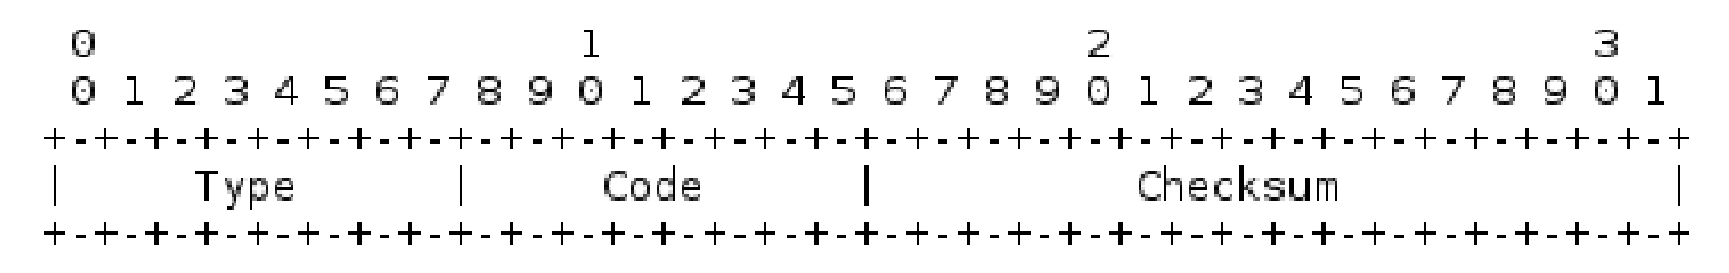
\includegraphics[width=15cm]{./pics/header.eps}
\\Le premier champ est celui de type. Il permet, premièrement, de donner le type du paquet et de l'information à transmettre, et deuxièmement de préciser la nature des champs qui vont suivres. En effet, comme vu plus haut, les messages contiennent des champs différents selon le type du message ICMP.
\\Le deuxième champ est le code. Il permet de subdiviser le type en donnant des détails plus précis.
\\Enfin le troisième champ est la somme de contrôle (checksum)//TODO(plage de controle).
\\Commençons avec les messages qui possèdent l'ensemble de champs le plus simple.

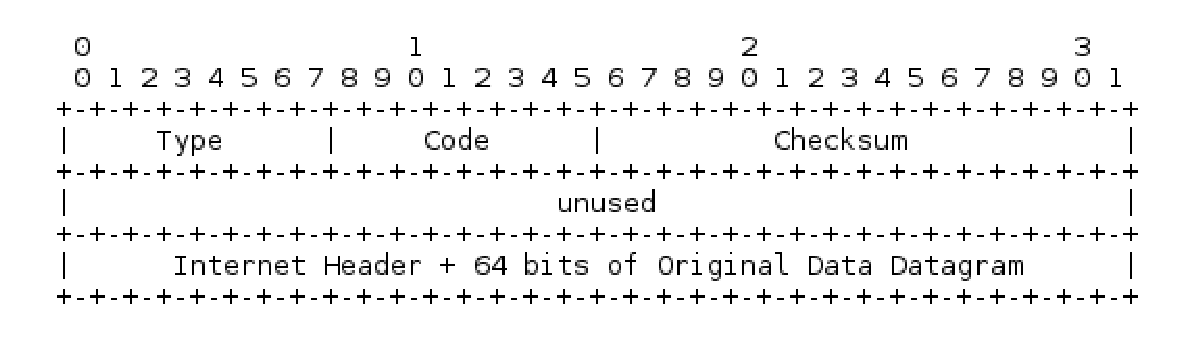
\includegraphics[width=15cm]{./pics/header1.eps}

\\Les messages qui utilisent cette organisation sont les messages de type 3, 4 et 11.
\subsubsection{Message de type 3: Unreachable Destination}
Les messages de type 3 sont émis lorsqu'un paquet n'a pas réussi à joindre la destination (Unreachable destination). Cette erreur peux être dut à plusieurs facteurs, et les codes permettent de préciser pourquoi le paquet n'a pas pu rejoindre sa destination.
\paragraph{Code 0}

\subsection{IGMP}
\subsection{DHCP}







\section{Lorem ipsum}

Lorem ipsum dolor sit amet, consectetur adipiscing elit. Nunc elementum nulla laoreet risus commodo, quis eleifend est ornare. Phasellus lobortis ex a lectus congue, ut posuere risus pellentesque. Mauris vitae nunc molestie, porta turpis a, ullamcorper ante. Etiam dictum risus justo, at sodales sem ultrices vel. Pellentesque a nisl vel justo molestie egestas a luctus lorem. Maecenas quam ante, volutpat non tempor non, tincidunt quis sem. Vivamus a lacus porttitor sem posuere finibus. Phasellus sed sapien quis quam ultricies condimentum.

Integer hendrerit nunc vitae luctus rutrum. Duis rhoncus, magna et aliquam lacinia, ante ex commodo nulla, in consequat odio augue vel odio. Vestibulum non odio varius ante sollicitudin condimentum sit amet et est. Proin ac dolor vitae ligula faucibus lobortis. Quisque dolor massa, lacinia ac tellus eget, ornare placerat diam. Fusce metus leo, molestie nec fringilla quis, sagittis ac libero. Nunc non turpis hendrerit, pellentesque orci sed, pretium sem. Vestibulum posuere, nunc eget sagittis molestie, enim arcu sagittis tellus, eu pharetra enim eros sit amet tellus. Aliquam scelerisque eleifend turpis, eu imperdiet quam posuere at. Aenean nec vulputate velit.

Nulla commodo, arcu id scelerisque finibus, massa ex dictum ex, id maximus eros nulla vel tortor. Aenean vulputate ante sed tellus consectetur, id hendrerit ligula bibendum. Fusce vestibulum ac nisl nec volutpat. Nam non lacus posuere, suscipit nisl non, feugiat tortor. Nunc commodo vulputate tristique. In interdum blandit nisl porta elementum. Nunc id nunc massa. Aenean cursus fermentum condimentum. Etiam eros nibh, finibus a dignissim nec, bibendum sit amet nunc. Vivamus accumsan blandit elit ut tristique. Suspendisse potenti. Aliquam id lectus sed purus eleifend fringilla. Integer eu libero vitae nulla imperdiet cursus sed et tellus. Proin porttitor interdum massa.

\subsection{Proin ullamcorper}

Proin ullamcorper id erat id ornare. Pellentesque ligula augue, aliquam vel consequat non, fringilla eget felis. Etiam nec luctus massa, a ullamcorper arcu. Sed ac ipsum ut velit maximus varius at tincidunt massa. Maecenas posuere bibendum molestie. Maecenas in turpis dui. Fusce nec accumsan lacus, tristique euismod magna. Morbi tristique nec magna a lacinia.

Suspendisse suscipit scelerisque nisi non iaculis. Mauris viverra rutrum nunc, nec lobortis arcu cursus non. Donec felis lectus, venenatis et lectus nec, faucibus dictum tortor. Pellentesque ac ipsum mi. Suspendisse sapien purus, imperdiet vel neque eu, sagittis suscipit justo. Suspendisse eu ornare lacus. Sed lobortis consequat mi id suscipit. Vestibulum a rutrum dolor, non hendrerit nulla. Phasellus felis nisi, maximus non augue eget, posuere iaculis sem. Ut ut tortor justo. Quisque turpis felis, finibus ut sem eget, commodo ullamcorper nisl. Cras a nulla euismod, placerat mauris nec, accumsan nunc. Vestibulum feugiat euismod justo vel pellentesque. Aliquam auctor est at libero elementum, quis sodales justo convallis. Proin lacus lacus, dignissim id est ac, cursus lacinia turpis.

Lorem ipsum dolor sit amet, consectetur adipiscing elit. Nunc elementum nulla laoreet risus commodo, quis eleifend est ornare. Phasellus lobortis ex a lectus congue, ut posuere risus pellentesque. Mauris vitae nunc molestie, porta turpis a, ullamcorper ante. Etiam dictum risus justo, at sodales sem ultrices vel. Pellentesque a nisl vel justo molestie egestas a luctus lorem. Maecenas quam ante, volutpat non tempor non, tincidunt quis sem. Vivamus a lacus porttitor sem posuere finibus. Phasellus sed sapien quis quam ultricies condimentum.

Integer hendrerit nunc vitae luctus rutrum. Duis rhoncus, magna et aliquam lacinia, ante ex commodo nulla, in consequat odio augue vel odio. Vestibulum non odio varius ante sollicitudin condimentum sit amet et est. Proin ac dolor vitae ligula faucibus lobortis. Quisque dolor massa, lacinia ac tellus eget, ornare placerat diam. Fusce metus leo, molestie nec fringilla quis, sagittis ac libero. Nunc non turpis hendrerit, pellentesque orci sed, pretium sem. Vestibulum posuere, nunc eget sagittis molestie, enim arcu sagittis tellus, eu pharetra enim eros sit amet tellus. Aliquam scelerisque eleifend turpis, eu imperdiet quam posuere at. Aenean nec vulputate velit.

Nulla commodo, arcu id scelerisque finibus, massa ex dictum ex, id maximus eros nulla vel tortor. Aenean vulputate ante sed tellus consectetur, id hendrerit ligula bibendum. Fusce vestibulum ac nisl nec volutpat. Nam non lacus posuere, suscipit nisl non, feugiat tortor. Nunc commodo vulputate tristique. In interdum blandit nisl porta elementum. Nunc id nunc massa. Aenean cursus fermentum condimentum. Etiam eros nibh, finibus a dignissim nec, bibendum sit amet nunc. Vivamus accumsan blandit elit ut tristique. Suspendisse potenti. Aliquam id lectus sed purus eleifend fringilla. Integer eu libero vitae nulla imperdiet cursus sed et tellus. Proin porttitor interdum massa.

Proin ullamcorper id erat id ornare. Pellentesque ligula augue, aliquam vel consequat non, fringilla eget felis. Etiam nec luctus massa, a ullamcorper arcu. Sed ac ipsum ut velit maximus varius at tincidunt massa. Maecenas posuere bibendum molestie. Maecenas in turpis dui. Fusce nec accumsan lacus, tristique euismod magna. Morbi tristique nec magna a lacinia.

\subsection{Suspendisse}

Suspendisse suscipit scelerisque nisi non iaculis. Mauris viverra rutrum nunc, nec lobortis arcu cursus non. Donec felis lectus, venenatis et lectus nec, faucibus dictum tortor. Pellentesque ac ipsum mi. Suspendisse sapien purus, imperdiet vel neque eu, sagittis suscipit justo. Suspendisse eu ornare lacus. Sed lobortis consequat mi id suscipit. Vestibulum a rutrum dolor, non hendrerit nulla. Phasellus felis nisi, maximus non augue eget, posuere iaculis sem. Ut ut tortor justo. Quisque turpis felis, finibus ut sem eget, commodo ullamcorper nisl. Cras a nulla euismod, placerat mauris nec, accumsan nunc. Vestibulum feugiat euismod justo vel pellentesque. Aliquam auctor est at libero elementum, quis sodales justo convallis. Proin lacus lacus, dignissim id est ac, cursus lacinia turpis.

Lorem ipsum dolor sit amet, consectetur adipiscing elit. Nunc elementum nulla laoreet risus commodo, quis eleifend est ornare. Phasellus lobortis ex a lectus congue, ut posuere risus pellentesque. Mauris vitae nunc molestie, porta turpis a, ullamcorper ante. Etiam dictum risus justo, at sodales sem ultrices vel. Pellentesque a nisl vel justo molestie egestas a luctus lorem. Maecenas quam ante, volutpat non tempor non, tincidunt quis sem. Vivamus a lacus porttitor sem posuere finibus. Phasellus sed sapien quis quam ultricies condimentum.

Integer hendrerit nunc vitae luctus rutrum. Duis rhoncus, magna et aliquam lacinia, ante ex commodo nulla, in consequat odio augue vel odio. Vestibulum non odio varius ante sollicitudin condimentum sit amet et est. Proin ac dolor vitae ligula faucibus lobortis. Quisque dolor massa, lacinia ac tellus eget, ornare placerat diam. Fusce metus leo, molestie nec fringilla quis, sagittis ac libero. Nunc non turpis hendrerit, pellentesque orci sed, pretium sem. Vestibulum posuere, nunc eget sagittis molestie, enim arcu sagittis tellus, eu pharetra enim eros sit amet tellus. Aliquam scelerisque eleifend turpis, eu imperdiet quam posuere at. Aenean nec vulputate velit.

Nulla commodo, arcu id scelerisque finibus, massa ex dictum ex, id maximus eros nulla vel tortor. Aenean vulputate ante sed tellus consectetur, id hendrerit ligula bibendum. Fusce vestibulum ac nisl nec volutpat. Nam non lacus posuere, suscipit nisl non, feugiat tortor. Nunc commodo vulputate tristique. In interdum blandit nisl porta elementum. Nunc id nunc massa. Aenean cursus fermentum condimentum. Etiam eros nibh, finibus a dignissim nec, bibendum sit amet nunc. Vivamus accumsan blandit elit ut tristique. Suspendisse potenti. Aliquam id lectus sed purus eleifend fringilla. Integer eu libero vitae nulla imperdiet cursus sed et tellus. Proin porttitor interdum massa.

Proin ullamcorper id erat id ornare. Pellentesque ligula augue, aliquam vel consequat non, fringilla eget felis. Etiam nec luctus massa, a ullamcorper arcu. Sed ac ipsum ut velit maximus varius at tincidunt massa. Maecenas posuere bibendum molestie. Maecenas in turpis dui. Fusce nec accumsan lacus, tristique euismod magna. Morbi tristique nec magna a lacinia.

Suspendisse suscipit scelerisque nisi non iaculis. Mauris viverra rutrum nunc, nec lobortis arcu cursus non. Donec felis lectus, venenatis et lectus nec, faucibus dictum tortor. Pellentesque ac ipsum mi. Suspendisse sapien purus, imperdiet vel neque eu, sagittis suscipit justo. Suspendisse eu ornare lacus. Sed lobortis consequat mi id suscipit. Vestibulum a rutrum dolor, non hendrerit nulla. Phasellus felis nisi, maximus non augue eget, posuere iaculis sem. Ut ut tortor justo. Quisque turpis felis, finibus ut sem eget, commodo ullamcorper nisl. Cras a nulla euismod, placerat mauris nec, accumsan nunc. Vestibulum feugiat euismod justo vel pellentesque. Aliquam auctor est at libero elementum, quis sodales justo convallis. Proin lacus lacus, dignissim id est ac, cursus lacinia turpis.

Lorem ipsum dolor sit amet, consectetur adipiscing elit. Nunc elementum nulla laoreet risus commodo, quis eleifend est ornare. Phasellus lobortis ex a lectus congue, ut posuere risus pellentesque. Mauris vitae nunc molestie, porta turpis a, ullamcorper ante. Etiam dictum risus justo, at sodales sem ultrices vel. Pellentesque a nisl vel justo molestie egestas a luctus lorem. Maecenas quam ante, volutpat non tempor non, tincidunt quis sem. Vivamus a lacus porttitor sem posuere finibus. Phasellus sed sapien quis quam ultricies condimentum.

Integer hendrerit nunc vitae luctus rutrum. Duis rhoncus, magna et aliquam lacinia, ante ex commodo nulla, in consequat odio augue vel odio. Vestibulum non odio varius ante sollicitudin condimentum sit amet et est. Proin ac dolor vitae ligula faucibus lobortis. Quisque dolor massa, lacinia ac tellus eget, ornare placerat diam. Fusce metus leo, molestie nec fringilla quis, sagittis ac libero. Nunc non turpis hendrerit, pellentesque orci sed, pretium sem. Vestibulum posuere, nunc eget sagittis molestie, enim arcu sagittis tellus, eu pharetra enim eros sit amet tellus. Aliquam scelerisque eleifend turpis, eu imperdiet quam posuere at. Aenean nec vulputate velit.

Nulla commodo, arcu id scelerisque finibus, massa ex dictum ex, id maximus eros nulla vel tortor. Aenean vulputate ante sed tellus consectetur, id hendrerit ligula bibendum. Fusce vestibulum ac nisl nec volutpat. Nam non lacus posuere, suscipit nisl non, feugiat tortor. Nunc commodo vulputate tristique. In interdum blandit nisl porta elementum. Nunc id nunc massa. Aenean cursus fermentum condimentum. Etiam eros nibh, finibus a dignissim nec, bibendum sit amet nunc. Vivamus accumsan blandit elit ut tristique. Suspendisse potenti. Aliquam id lectus sed purus eleifend fringilla. Integer eu libero vitae nulla imperdiet cursus sed et tellus. Proin porttitor interdum massa.

Proin ullamcorper id erat id ornare. Pellentesque ligula augue, aliquam vel consequat non, fringilla eget felis. Etiam nec luctus massa, a ullamcorper arcu. Sed ac ipsum ut velit maximus varius at tincidunt massa. Maecenas posuere bibendum molestie. Maecenas in turpis dui. Fusce nec accumsan lacus, tristique euismod magna. Morbi tristique nec magna a lacinia.

Suspendisse suscipit scelerisque nisi non iaculis. Mauris viverra rutrum nunc, nec lobortis arcu cursus non. Donec felis lectus, venenatis et lectus nec, faucibus dictum tortor. Pellentesque ac ipsum mi. Suspendisse sapien purus, imperdiet vel neque eu, sagittis suscipit justo. Suspendisse eu ornare lacus. Sed lobortis consequat mi id suscipit. Vestibulum a rutrum dolor, non hendrerit nulla. Phasellus felis nisi, maximus non augue eget, posuere iaculis sem. Ut ut tortor justo. Quisque turpis felis, finibus ut sem eget, commodo ullamcorper nisl. Cras a nulla euismod, placerat mauris nec, accumsan nunc. Vestibulum feugiat euismod justo vel pellentesque. Aliquam auctor est at libero elementum, quis sodales justo convallis. Proin lacus lacus, dignissim id est ac, cursus lacinia turpis.

\section{Conclusion}
\label{sec:ccl}
Comme indiqué dans la section~\ref{sec:intro}, ce document peut servir de modèle pour un rapport d'étude.

\cleardoublepage
\addcontentsline{toc}{section}{Références}
\bibliographystyle{plain}
\bibliography{rapport}

\end{document}
